%%
% BIThesis Undergraduate Thesis Template (English) — Compile with XeLaTeX
% Chapter 3: System Implementation and Data Design
%%

\chapter{System Implementation and Data Design}

This chapter details the concrete engineering implementation of the SDN control plane. To transition the high-level architecture into a functional distributed system, careful consideration must be given to data persistence, inter-service communication contracts, and core algorithmic logic. This chapter unpacks the Atomix database deployment, the internal entity-relationship models, the Protocol Buffer telemetry pipeline, the mathematical implementation of the auction logic, and the simulated boundary components.

\section{Distributed Consensus Storage Design}

The control plane relies entirely on Atomix as its single source of truth. Because multiple microservices (API Gateway, Auction Runner, Telemetry Processor) concurrently read and write to this state, a standard relational database is insufficient. The system implements a distributed consensus store based on the Raft consensus algorithm to guarantee linearizable reads and writes across the cluster.

\subsection{Atomix Cluster Configuration}
To ensure high availability and partition tolerance, the Atomix cluster is deployed natively within Kubernetes using a Custom Resource Definition (CRD). The configuration explicitly provisions a multi-replica Raft group. 

As defined in the system's \texttt{store.yaml} configuration (Figure~\ref{lst:atomix_store}), the \texttt{ConsensusStore} is configured with \texttt{replicas: 3} and \texttt{groups: 3}. This specific replication factor ensures that the cluster can tolerate the failure of a minority node while maintaining a strict quorum for leader election and log replication. Furthermore, the storage class dynamically provisions 8Gi of persistent block storage per node to ensure transaction logs survive container restarts.

\begin{figure}[H]
\begin{minted}[fontsize=\scriptsize, frame=single]{yaml}
apiVersion: consensus.atomix.io/v1beta1
kind: ConsensusStore
metadata:
  name: consensus-store
spec:
  replicas: 3
  groups: 3
  volumeClaimTemplate:
    spec:
      accessModes:
        - ReadWriteOnce
      volumeMode: Filesystem
      resources:
        requests:
          storage: 8Gi
      storageClassName: standard
\end{minted}
\caption{The Kubernetes deployment configuration for the Atomix Consensus Store, specifying a 3-node fault-tolerant Raft architecture.}
\label{lst:atomix_store}
\end{figure}

The microservices bind to this cluster using a \texttt{StorageProfile}, which abstracts the physical pod IP addresses into a logical routing layer, allowing the Go microservices to connect seamlessly via gRPC.

\section{Core Data Models and Schema Design}

To support the dynamic auction marketplace, the Atomix key-value store manages several core data structures. Because Atomix operates as a NoSQL document store, these entities are defined as serialized Go structs and stored as byte arrays. The relationships between these entities are illustrated in Figure~\ref{fig:er_diagram}.

%%% ADVISOR TIP: Draw a simple ER diagram showing Customer -> Bid -> Allocation %%%
\begin{figure}[H]
  \centering
  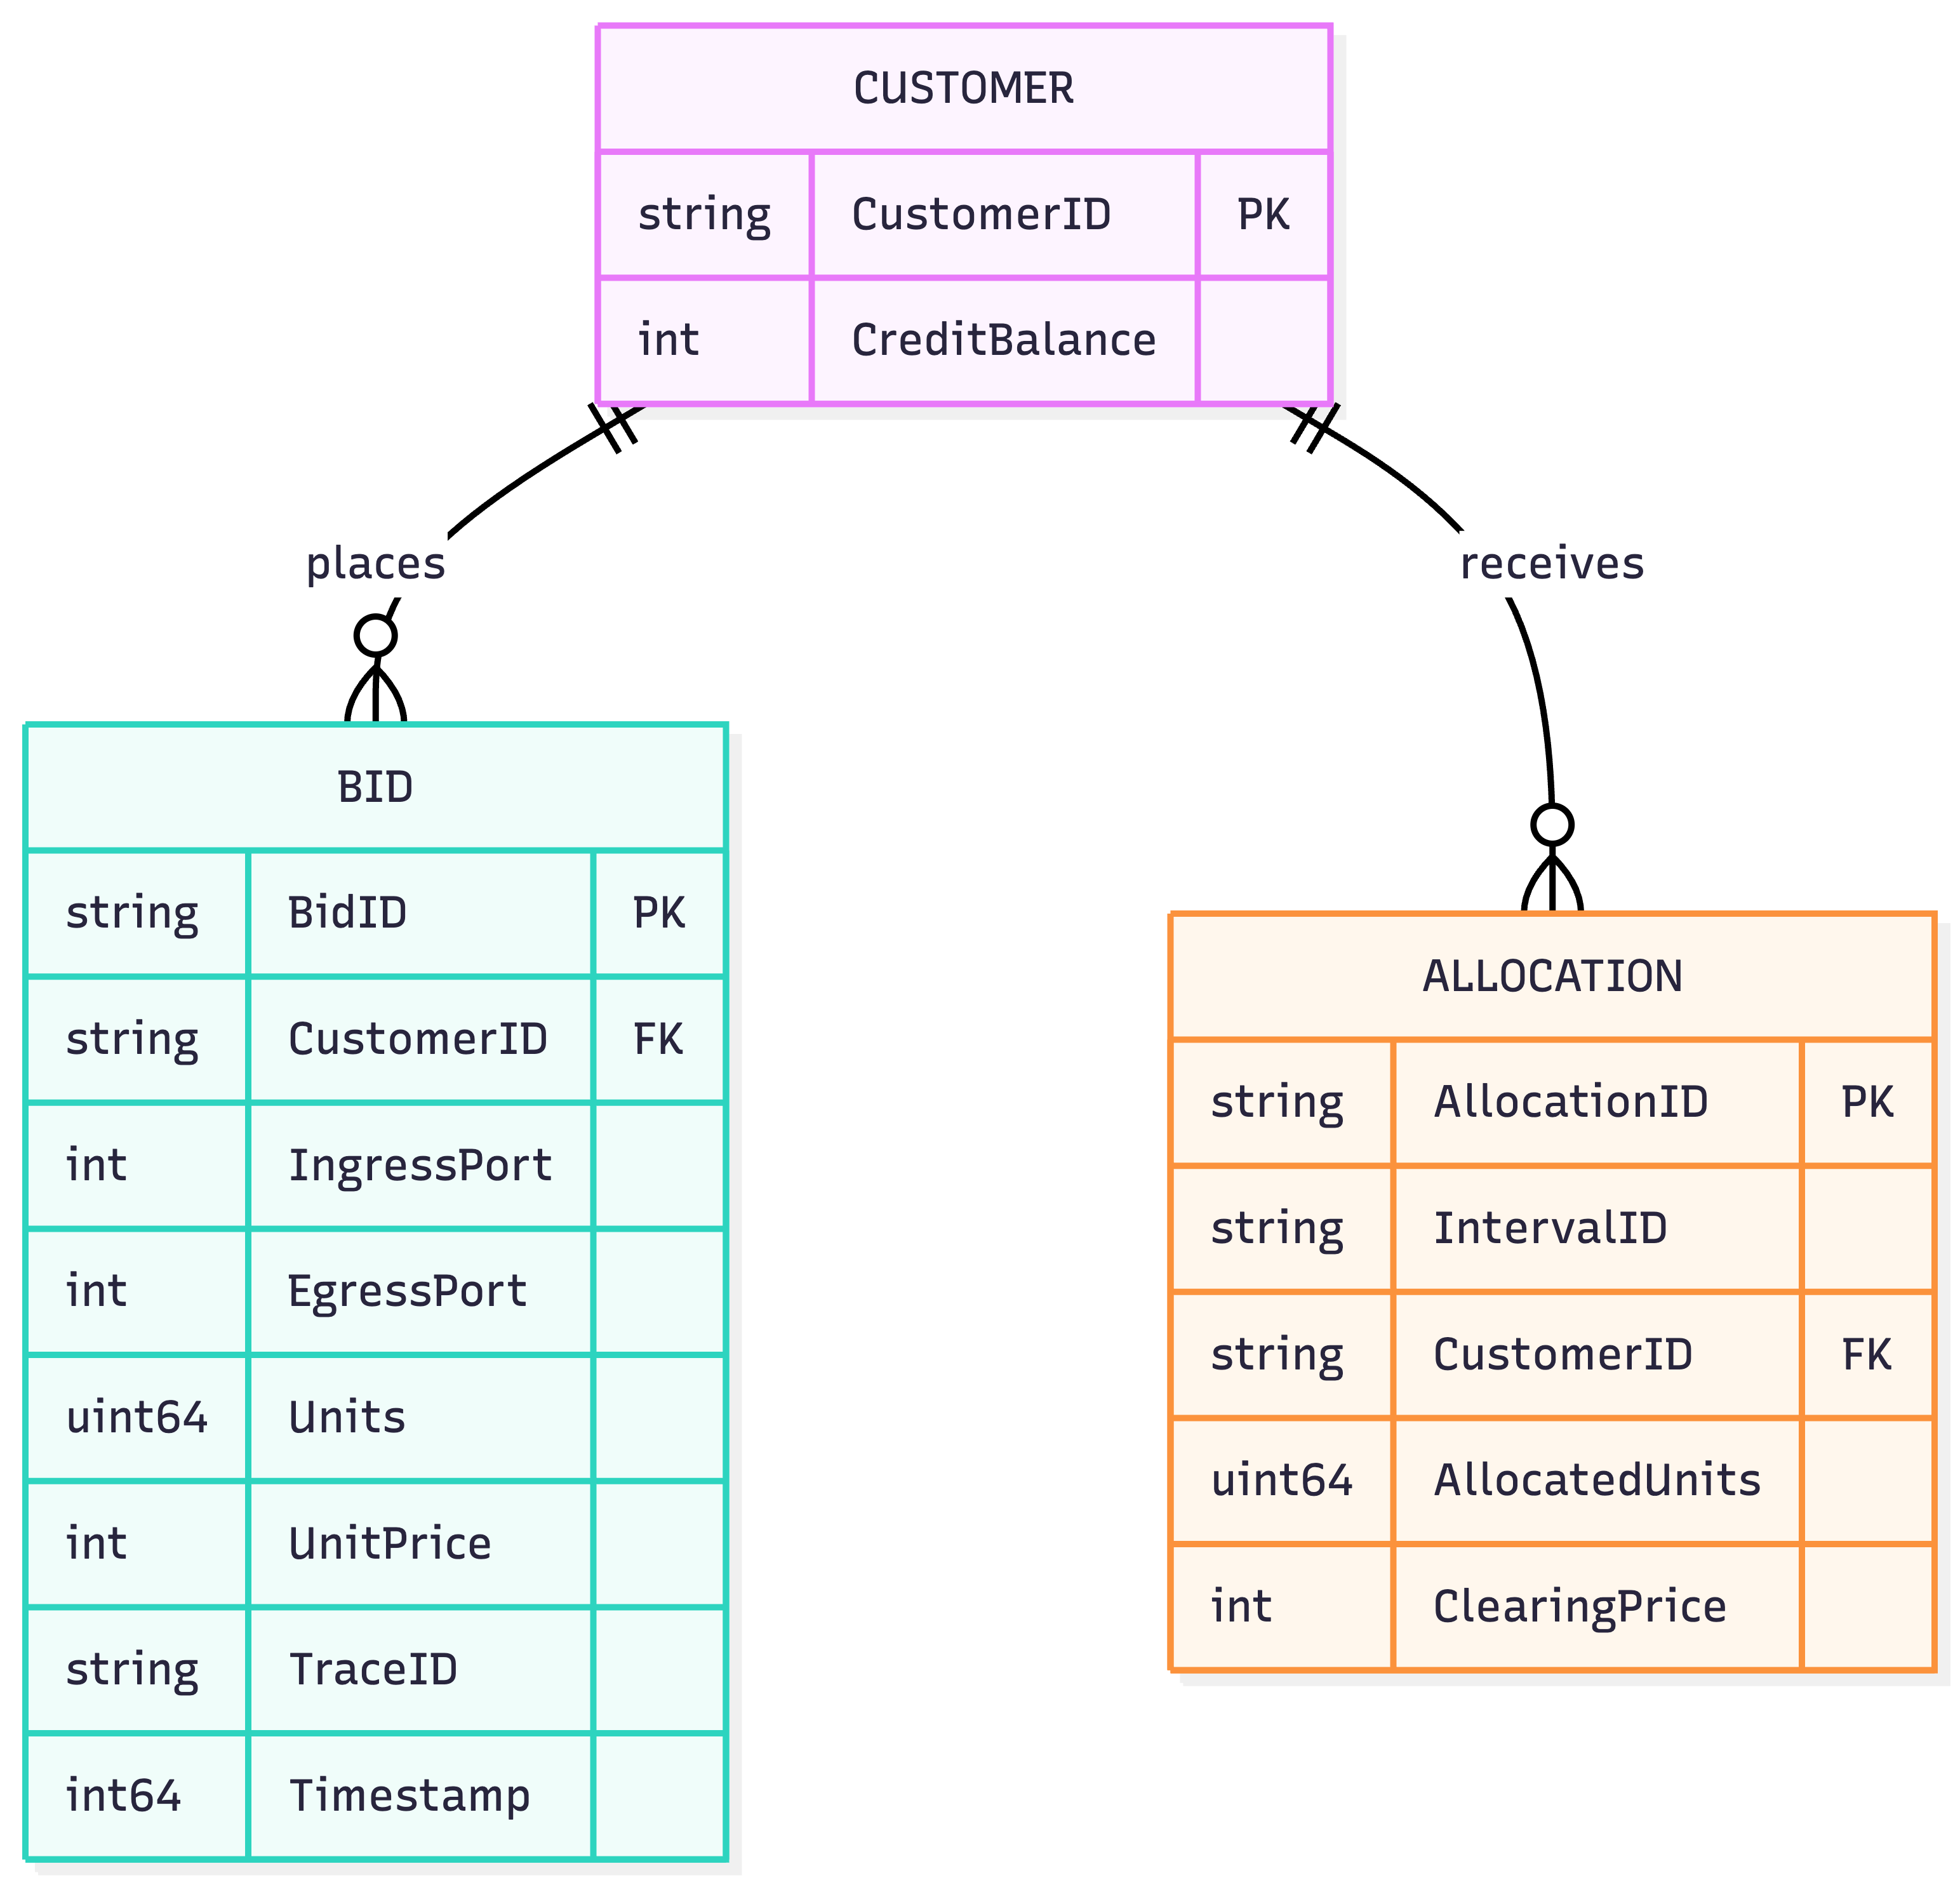
\includegraphics[width=0.85\textwidth]{images/er-diagram.png}
  \caption{Entity-Relationship diagram of the core control plane data structures.}
  \label{fig:er_diagram}
\end{figure}

\subsection{Bid Entity Schema}
The \texttt{Bid} entity represents a customer's intent to purchase bandwidth for a specific network path. The API Gateway validates incoming HTTP requests and constructs this entity before committing it to Atomix. Table~\ref{tab:schema_bid} details the schema fields.

\begin{table}[H]
\centering
\caption{Database Schema: Bid Entity}
\label{tab:schema_bid}
\begin{tabular}{llp{8cm}}
\toprule
\textbf{Field Name} & \textbf{Data Type} & \textbf{Description} \\
\midrule
\texttt{BidID} & String (UUID) & Primary Key. Uniquely identifies the bid transaction. \\
\texttt{CustomerID} & String & Foreign Key linking to the originating AS agent. \\
\texttt{IngressPort} & Integer & The network entry point for the traffic flow. \\
\texttt{EgressPort} & Integer & The congested bottleneck port being auctioned. \\
\texttt{Units} & Unsigned Int64 & Requested bandwidth volume in Kbps. \\
\texttt{UnitPrice} & Integer & Maximum willingness to pay per unit of bandwidth. \\
\texttt{TraceID} & String & Injected OpenTelemetry trace context carrier. \\
\texttt{Timestamp} & Epoch (Int64) & Unix timestamp of ingestion for interval filtering. \\
\bottomrule
\end{tabular}
\end{table}

\subsection{Allocation and Credit History Schemas}
Once the Auction Runner computes the clearing algorithm, it generates \texttt{Allocation} records and updates the customer's \texttt{Credit} profile. Tracking credit ensures that agents operate within a finite budget, preventing malicious actors from continuously submitting infinite bids to monopolize the network. Table~\ref{tab:schema_allocation} details the Allocation schema.

\begin{table}[H]
\centering
\caption{Database Schema: Allocation Entity}
\label{tab:schema_allocation}
\begin{tabular}{llp{8cm}}
\toprule
\textbf{Field Name} & \textbf{Data Type} & \textbf{Description} \\
\midrule
\texttt{AllocationID} & String (UUID) & Primary Key for the granted bandwidth reservation. \\
\texttt{IntervalID} & String & Links the allocation to a specific 30s auction round. \\
\texttt{CustomerID} & String & Identifies the recipient of the bandwidth. \\
\texttt{AllocatedUnits} & Unsigned Int64 & Final granted bandwidth (may be less than requested). \\
\texttt{ClearingPrice} & Integer & The uniform market price applied to the allocated units. \\
\bottomrule
\end{tabular}
\end{table}

The system maintains an \texttt{AuctionHistory} ledger for each customer. At the end of every interval, the total cost (\texttt{AllocatedUnits} $\times$ \texttt{ClearingPrice}) is deducted from the customer's active credit balance. If an agent exhausts its credits, the API Gateway rejects its future bids with an HTTP 402 Payment Required status.

\section{Inter-Service Communication Protocols}

In a decoupled microservice architecture, the choice of data serialization format significantly impacts system latency and network throughput. While the API Gateway utilizes standard JSON over HTTP for external customer interactions, internal asynchronous communication via Apache Kafka requires a highly optimized binary format. 

To satisfy this requirement, the control plane utilizes Google Protocol Buffers (Protobuf) for all internal message passing. Protobuf provides a strictly typed, language-agnostic contract between services, ensuring backward compatibility and significantly smaller payload sizes compared to JSON.

\subsection{Data Plane Telemetry Contracts}
The most high-frequency communication path in the system is the telemetry pipeline, where the simulated data plane continuously streams network statistics back to the control plane. This contract is defined by the \texttt{flow.proto} schema. 

As detailed in Table~\ref{tab:proto_flow}, the base unit of network measurement is the \texttt{FlowDigest}. Because physical network switches operate at line rate, they do not inherently understand higher-level metrics like ``Kilobits per second'' (Kbps). Instead, they maintain hardware counters of absolute bytes transferred for a given ingress-egress port pair. The \texttt{TelemetryReport} wraps multiple flow digests into a single timestamped batch to minimize Kafka producer overhead.

\begin{table}[H]
\centering
\caption{Protobuf Schema: Data Plane Telemetry Report (\texttt{flow.proto})}
\label{tab:proto_flow}
\begin{tabular}{llp{8cm}}
\toprule
\textbf{Message} & \textbf{Field} & \textbf{Description} \\
\midrule
\texttt{FlowDigest} & \texttt{ingress\_port} & (uint64) The physical entry port of the traffic. \\
& \texttt{egress\_port} & (uint64) The physical exit port of the traffic. \\
& \texttt{bytes\_transferred} & (uint64) Absolute counter of bytes routed. \\
& \texttt{packets\_dropped} & (uint64) Counter of packets dropped due to congestion. \\
\midrule
\texttt{TelemetryReport} & \texttt{switch\_id} & (string) Unique identifier of the reporting hardware. \\
& \texttt{timestamp} & (int64) Unix epoch time of the hardware snapshot. \\
& \texttt{flows} & (repeated FlowDigest) Array of flow counters. \\
\bottomrule
\end{tabular}
\end{table}

\section{Network Telemetry Processing Pipeline}

While the Auction Runner handles the economic allocation of bandwidth, the marketplace cannot function unless bidding agents have access to real-time network congestion data. The Telemetry Processing Pipeline is responsible for transforming the raw, absolute hardware counters into actionable, relative flow rates.

\subsection{State Aggregation and Rate Calculation}
The Telemetry Processor microservice operates as a continuous Kafka consumer, subscribed to the \texttt{switch-telemetry} topic. Upon ingesting a \texttt{TelemetryReport} protobuf message, the processor deserializes the byte payload and begins the aggregation phase.

Because the switch only provides absolute byte counters, the processor must maintain state to calculate the current flow rate. The system queries the Atomix consensus store to retrieve the previous byte count and timestamp for a specific flow. The real-time throughput is then derived using the following rate equation:

\begin{equation}
    \text{Throughput (Kbps)} = \frac{(\text{CurrentBytes} - \text{PreviousBytes}) \times 8}{(\text{CurrentTime} - \text{PreviousTime})} \times \frac{1}{1000}
\end{equation}

\subsection{Flow State Persistence}
Once the relative throughput and packet drop rates are calculated, the Telemetry Processor marshals this derived data back into a structured Go entity (\texttt{FlowMetrics}). This entity is subsequently committed back into the Atomix consensus store under a hierarchical routing key format. By persisting this derived state into Atomix, the architecture achieves a highly efficient read-path. When a Customer Agent prepares to formulate a bid, it performs a direct, low-latency read from the Atomix key-value store, bypassing the heavy computational overhead of the Kafka streams. 

\section{Auction Clearing Implementation}

The Auction Runner acts as the economic engine of the system. Rather than reacting to customer requests synchronously, it utilizes an interval-triggered batch processing model as illustrated in (Figure~\ref{fig:auction_flowchart}) to compute fair bandwidth allocations, querying the Atomix state store to process bids collectively.

%%% ADVISOR TIP: Draw a flowchart showing the Auction Runner loop %%%
\begin{figure}[H]
  \centering
  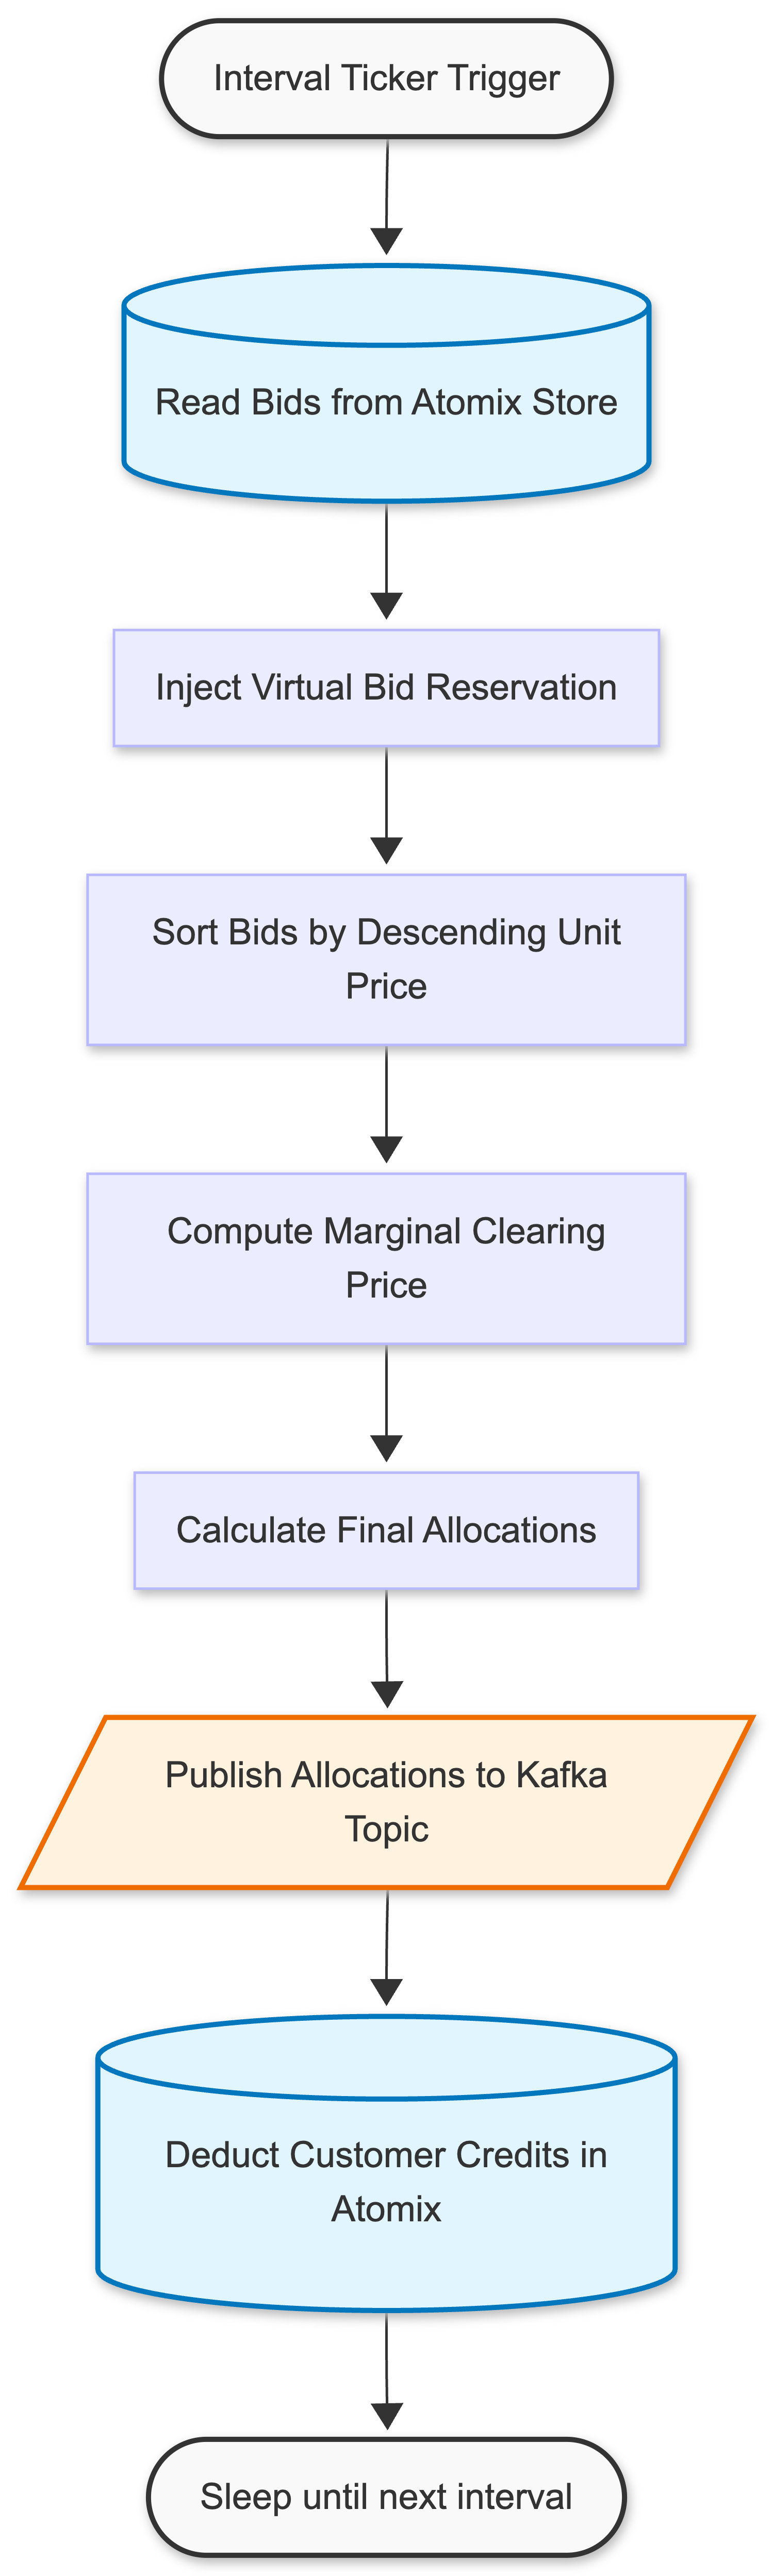
\includegraphics[width=0.30\textwidth]{images/auction-flowchart.png}
  \caption{Execution flow of the Auction Runner, detailing the interval trigger, state retrieval, clearing computation, and asynchronous result publication.}
  \label{fig:auction_flowchart}
\end{figure}

\subsection{The Uniform-Price Mathematical Formulation}
At each interval trigger, the runner executes a sealed-bid, uniform-price auction. Let the total available bandwidth capacity for a specific egress port be denoted as $C$. The system retrieves a set of $n$ eligible bids $B = \{b_1, b_2, \dots, b_n\}$ from Atomix. Each bid $b_i$ is represented as a tuple $(q_i, p_i)$, where $q_i$ denotes the requested bandwidth quantity (\texttt{Units}) and $p_i$ represents the maximum willingness to pay (\texttt{UnitPrice}).

To execute the auction, the algorithm first sorts the bids in descending order of price, such that $p_1 \ge p_2 \ge \dots \ge p_n$. 

\textbf{Clearing Price Determination:}
The algorithm iterates through the sorted bids, accumulating the demanded quantity until the capacity $C$ is exhausted. The clearing price $P^*$ is defined by the price of the marginal bid $k$ where the cumulative demand meets or exceeds capacity:
\begin{equation}
    P^* = p_k \quad \text{where} \quad \sum_{i=1}^{k-1} q_i < C \quad \text{and} \quad \sum_{i=1}^{k} q_i \ge C
\end{equation}
If the total demand is strictly less than the capacity ($\sum q_i < C$), the clearing price defaults to the price of the lowest submitted bid ($P^* = p_n$).

\textbf{Allocation Rule:}
Let $x_i$ denote the final bandwidth allocated to bid $b_i$. The allocation is divided into three tiers based on the clearing price:
\begin{enumerate}
    \item \textbf{Inframarginal Bids ($p_i > P^*$):} These bids clear the market and are fully allocated. 
    \begin{equation}
        x_i = q_i
    \end{equation}
    \item \textbf{Extramarginal Bids ($p_i < P^*$):} These bids fail to clear the market and are rejected. 
    \begin{equation}
        x_i = 0
    \end{equation}
    \item \textbf{Marginal Bids ($p_i = P^*$):} These bids tie exactly at the clearing price. Let $M = \{j \mid p_j = P^*\}$ be the set of marginal bids, and $D_M = \sum_{j \in M} q_j$ be their total demand. The remaining capacity available for these marginal bids is $C_{rem} = C - \sum_{i : p_i > P^*} q_i$. Marginal bids receive a strictly proportional share of the remaining capacity:
    \begin{equation}
        x_i = \min \left( q_i, \quad q_i \times \frac{C_{rem}}{D_M} \right) \quad \forall i \in M
    \end{equation}
\end{enumerate}

\subsection{Reservation Price Extension via Virtual Bidding}
To prevent bandwidth from being sold at unsustainably low prices during periods of low demand, the algorithm must support a strict Reservation Price ($R$).

Rather than introducing complex branching logic into the core algorithm, the reservation price is elegantly implemented via a \textit{Virtual Bid injection}. Before the sorting phase, the Go implementation automatically generates a virtual bid $b_v = (C, R)$—requesting the entire link capacity at the minimum reservation price—and appends it to the bid set $B$.

The standard uniform-price sorting and clearing equations are then executed on this augmented set $B \cup \{b_v\}$. This mathematically guarantees that the clearing price $P^*$ is strictly bounded: $P^* \ge R$. Crucially, during the proportional allocation phase for marginal bids (if $P^* = R$), the algorithm excludes the virtual bid from the marginal demand calculation ($D_M$), ensuring that the virtual bid successfully establishes a price floor without artificially diluting the proportional allocation share of genuine customer bids.

\section{Test Environment Simulation}

To rigorously test the mathematical clearing algorithm and the telemetry processing pipeline without the overhead or latency of physical network hardware, the system implements simulated boundary components written in Go.

\subsection{The Simulated Agent (Bid Simulator)}
The Simulated Agent acts as the upstream customer. It is implemented as a high-throughput load generator capable of reading from configuration-driven scenario files (YAML) to simulate various market conditions, such as diurnal traffic spikes or sudden port congestion. By continuously firing HTTP POST requests at the API Gateway, it stresses the Atomix write-throughput and validates the robustness of the auction algorithm under heavy concurrent load.

\subsection{The Simulated Switch (Telemetry Simulator)}
The Simulated Switch acts as the downstream data plane. It connects directly to the Kafka cluster to consume the final \texttt{auction-results} messages generated by the algorithm. Simultaneously, it runs a background goroutine that generates simulated flow digests (representing hardware byte counters) and publishes them to the \texttt{switch-telemetry} topic every second. This isolates the control plane logic, ensuring that any evaluated performance benchmarks reflect software efficiency rather than physical switch hardware limitations.

\section{Summary}

This chapter detailed the logical implementation and data design of the control plane's core functionalities. By explicitly defining the Atomix consensus storage, the protobuf contracts, and the mathematical telemetry processing, the system is proven to be robust and highly scalable. The auction algorithm utilizes formal mathematical uniform-pricing to ensure fair bandwidth allocation, successfully enhanced by a virtual-bid software mechanism to enforce reservation pricing. 

While the economic logic and data pipelines are now firmly established, operating these asynchronous microservices in production requires deep systemic visibility. The next chapter presents the Observability Framework, detailing how the system is instrumented to track these complex algorithms and expose distributed failures.